\section{Hormigas}
%\subsection{Metaheur\'istica ACO }
\begin{frame}{Hormigas (OE 1)}
    \centering
    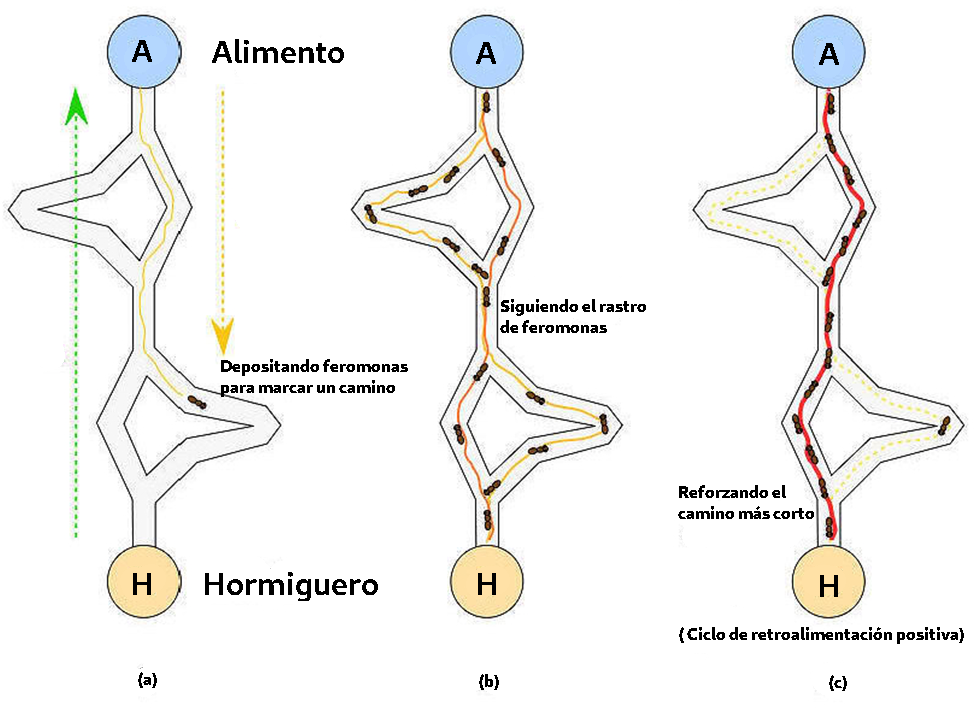
\includegraphics[height=2.5in]{Pictures/ACO-ant.png}
\end{frame}

\note[itemize]{
    \item Como se mencion\'o previamente, uno de los problemas principales al individualizar filamentos es que se desconoce el comienzo y el final de un filamento al comienzo del problema. 
    \item As\'i, resulta natural explorar el comportamiento de las hormigas al buscar alimento como inspiraci\'on para individualizar filamentos
    \item A la izquierda de la imagen, en la letra {\bf a}, se puede observar que una hormiga que sale del hormiguero recorre un camino aleatorio hasta llegar al alimento. En su retorno, por el mismo camino, deposita feromonas para indicarle a otras hormigas por donde fue su recorrido.
    
    \item Luego, otras hormigas pueden tomar esta informaci\'on en su propio descubrimiento de un camino hacia el alimento, como se observa el la mitad de la imagen, en {\bf b}
    
    \item Finalmente, a la derecha de la imagen, se observa que las hormigas depositan m\'as y m\'as feromonas en el camino m\'as corto entre el hormiguero y el alimento, causando una convergencia sobre un camino \'optimo. Esta convergencia es lo que se define como el ciclo de reforzamiento positivo

}



\begin{frame}{Modelo de Feromonas (OE 1)}
\small
\begin{itemize}
    \item Comunicaci\'on indirecta mediante feromonas
    \item Recorrido aleatorio
    \item Convergencia sobre el camino m\'as corto
    \item Opciones de caminos posibles representan el espacio de b\'usqueda
\end{itemize}
    \begin{algorithm}[H]
    \SetAlgoLined
     Ajuste de Par\'ametros \& inicializaci\'on de feromonas\;
     \While{Criterio de finalizaci\'on no se cumple}{
       Construcci\'on\_de\_soluci\'on\_de\_cada\_hormiga()\;
       M\'etodo\_de\_b\'usqueda\_no\_local(); //Paso opcional\\
       Actualizaci\'on\_de\_feromonas()\;
     }
     \caption{Algoritmo metaheur\'istica ACO}\label{ACO-Algo}
    \end{algorithm}
\end{frame}

\note[itemize]{
    \item El comportamiento anterior se puede describir como el modelo de feromonas, 
    \item Orden no estricto
}

\begin{frame}{Etapas del Algoritmo Propuesto (OE 1)}
\centering  
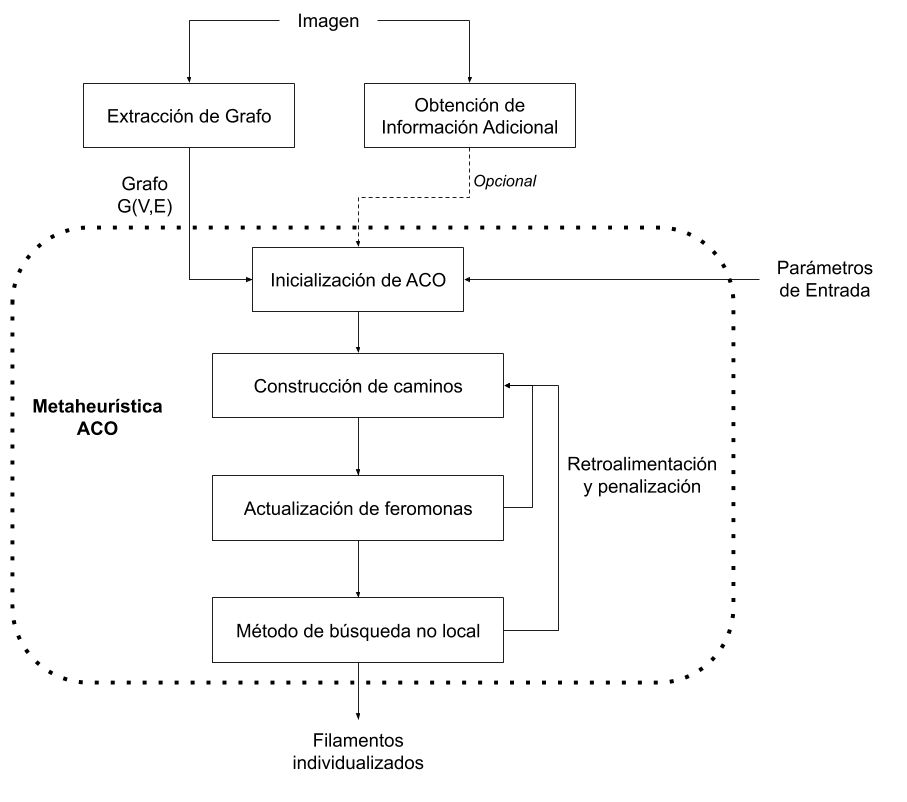
\includegraphics[height=2.5in]{Pictures/ACOdiagram.png}
\end{frame}

\note[itemize]{
    \item Diagrama de las etapas del algoritmo propuesto
}

%\subsection{Problema de Satisfacci\'on de Restricciones}
% \begin{frame}{ACO aplicado como Problema de Satisfacci\'on de Restricciones (OE 1)}
%   \begin{columns}
%     \begin{column}{0.5\textwidth}
%         \begin{itemize}
%           \item $P = (S, \Omega, F)$
%           % esta definido por un conjunto discreto de variables
%           \item S:  Cjto. de soluciones, compuesto por variables discretas $X_{i}$, $i \in 1 \dotsc n$
%           %\item $S:\quad X = v_{i}^{j} \in D_{i} = \{v_{i}^{1} \dotsc  v_{i}^{|D_{i}|}\}$.
%           \item Sol. Candidata $s \in S$, y $s^{*}$ una soluci\'on \'optima
%           \item Cjto. de Restricciones $\Omega$
%           \item Funci\'on objetivo $F: S\rightarrow \mathbb R_{0}^{+}$
%           %\item  
          
%       \end{itemize}
%     \end{column}
%     \begin{column}{0.5\textwidth}
%       \begin{itemize}
%           \item $s$ es factible si satisface las restricciones de $\Omega$
%           % y se relacionan mediante 
%           \item Pueden existir m\'ultiples soluciones $s^{*}$
%           \item $S^{*}$ es el conjunto que engloba todas las soluciones \'optimas
%           \item $s^{*} \in S^{*} \subseteq S$
%       \end{itemize}
%     \end{column}
% \end{columns}
% \end{frame}





% \begin{frame}{Adaptaci\'on a Individualizaci\'on de Filamentos}
%     \begin{algorithm}[H]
%     \SetAlgoLined
%     \KwData{Variables $X_i \dotsc X_n$, dominios $D_1 \dotsc D_n$, Restricciones $\in \Omega$}
%     \KwResult{conjunto s\textquotesingle $ \subseteq S$ != $\emptyset$, si existen soluciones factibles}
%      Ajuste de Par\'ametros \& inicializaci\'on de feromonas \;
%      \While{Criterio de finalización no se cumple}{
%       Construcci\'on\_de\_soluci\'on\_de\_cada\_hormiga()\;
%       M\'etodo\_de\_b\'usqueda\_no\_local(); //Paso opcional\\
%       Actualizaci\'on\_de\_feromonas()\;
%      }
%      \caption{Algoritmo de un modelo COP adaptado a una metaheur\'istica ACO}\label{COP-ACO-Algo}
%     \end{algorithm}
% \end{frame}


\section{Algoritmo Propuesto}



%\subsection{Construcci\'on de Soluciones}
\begin{frame}{ACO: Construcci\'on de Soluci\'on (OE 1)}
\centering
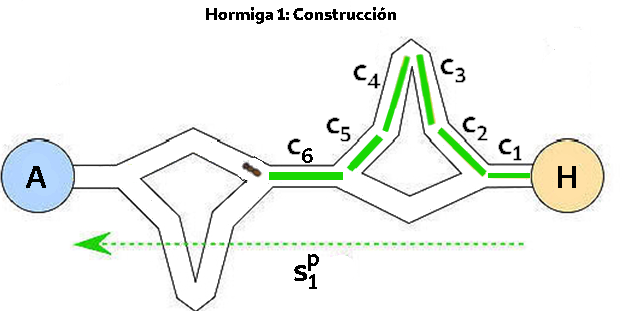
\includegraphics[scale=0.4]{Pictures/ACO-ant-Constr.png}
\begin{itemize}
    \item Influencia de feromonas $\tau$ y de una heur\'istica $\eta$ en la elecci\'on de Aristas/Componentes $c_i$ que respeten restricciones en $\Omega$
    \item Aspecto aleatorio en la elecci\'on
\end{itemize}
\end{frame}

% \begin{frame}{ACO: Heur\'istica de Asignaci\'on Inicial}
% \begin{enumerate}
% \item Arista $a: (n_i,n_j)$ tal que $deg(n_i) = 1$ o $deg(n_j) = 1$ 
% %La arista a asignar debe tener al menos uno de sus nodos con grado 1, indicando que es el inicio o final de una parte del grafo.

% \item De no haber aristas disponibles con esas caracter\'isticas, se realiza una asignaci\'on inicial de una arista que cumpla con 2 criterios:
% \begin{itemize}
%     \item $a: (n_i,n_j)$ tal que $deg(n_i) >= 2$ o $deg(n_j) >= 2$ 
%     \item El \'angulo que forma la arista candidata a elegir, junto a otra arista a la que pertenece el nodo, debe pertenecer al rango $]\theta, Max\_Angle]$.
% \end{itemize}

% \item Una arista aleatoria que no pertenezca a una soluci\'on o camino evaluado como de buena calidad
% %. La calidad de un camino se presenta m\'as adelante en esta secci\'on.
% \end{enumerate}
% \end{frame}

\begin{frame}{ACO: Construcci\'on de Soluci\'on, Asignaci\'on de 1ra Arista (OE 1)}
    \begin{columns}
        \begin{column}{0.35\textwidth}
            \begin{itemize}
                \item Heur\'istica de Asignaci\'on Inicial: \begin{enumerate}
                    \item Arista con un nodo grado 1
                    \item Aristas en intersecciones
                    \item Arista aleatoria
                \end{enumerate}
                
            \end{itemize}
        \end{column}
        \begin{column}{0.65\textwidth}
            \centering
            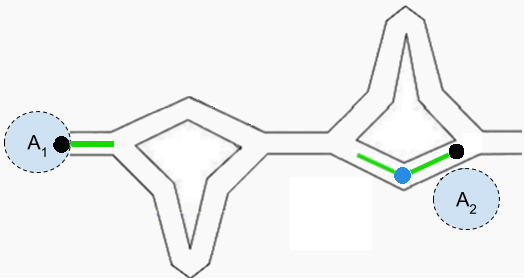
\includegraphics[scale=0.5]{Pictures/ant-initial-edge.png}
        \end{column}
    \end{columns}
\end{frame}

\note[itemize]{
    \item Al comenzar, se debe asignar una arista. Para esto, se propone una heur\'istica que consta de 3 criterios. El enfoque de estos criterios se centra en la exploraci\'on del espacio de b\'usqueda
    \item El primer criterio busca asignar aristas que esten en el borde del grafo
    
    \item De no existir m\'as aristas como las del 1er criterio, se buscan aristas que se encuentren en intersecciones, es decir que tengan uno de sus nodos con grado 2 o superior, y que el angulo que formen las aristas que comparten aquel nodo este en el rango intermedio definido previamente. Esto debido a que en varios tipos de filamentos hay casos en que los filamentos no nacen s\'olo del borde, sino tambi\'en a partir de otros filamentos.
    
    \item Como criterio final, se elige una arista al azar, privilegiando las aristas que no son parte de un camino ya evaluado como de buena calidad.

}


\begin{frame}{ACO: Construcci\'on de Soluci\'on (OE 1)}
    \begin{columns}
        \begin{column}{0.7\textwidth}
            \centering
            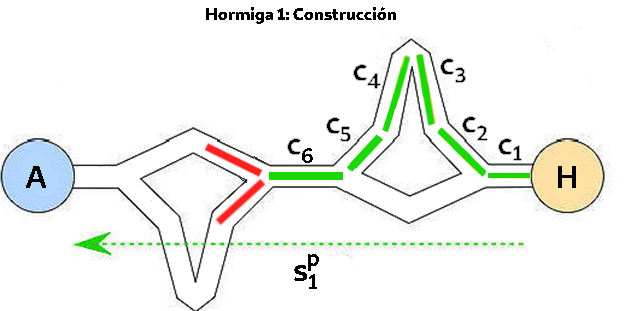
\includegraphics[scale=0.4]{Pictures/ACO-ant-Constr-choices.png}
        \end{column}
        \begin{column}{0.3\textwidth}
            \begin{equation}
            P(c_{i} | s^{P}) = \frac
            {\tau_{i} ~ \eta_{i}}
            {\sum\limits_{c_{j}\in N(s^p)}{\tau_{j} ~ \eta_{j} } } %, \forall c_{i} \in N(s^{P}).
            \label{eq:antProbabilities}
            \end{equation}
        \end{column}
    \end{columns}

    \begin{columns}
        \begin{column}{0.35\textwidth}
            \begin{itemize}
                \item Calidad $\sim$ Funci\'on Objetivo 
                \item Calidad $s^{P}_1$ = $\sum \eta_{i}$
                \item Calidad $s_1$ = $\frac{1}{n}\sum \eta_{i} $
            \end{itemize}
        \end{column}
        \begin{column}{0.65\textwidth}
            \begin{itemize}%\fontsize{9pt}{10}\selectfont
                \item Calidad M\'inima $\geq \frac{Max\_Score}{2}$
                \item Buena Calidad: $Max\_Score$
                \item Calidad Intermedia: $[\frac{Max\_Score}{2}, Max\_Score[$
            \end{itemize}
        \end{column}
    \end{columns}
\end{frame}

\note[itemize]{
    \item Para evaluar la construcci\'on del camino, se suman los valores de la heur\'istica miope de cada arista seleccionada.
    
    As\'i, al referirnos a la calidad de una soluci\'on, nos referimos al valor entregado por la funci\'on objetivo. Se busca maximizar la funci\'on objetivo. 

}

%\subsection{M\'etodo de b\'usqueda no local}
\begin{frame}{B\'usqueda no local: l\'ogicas globales/centralizadas (OE 1)}
    
    \begin{columns}
        \begin{column}{0.4\textwidth}
            \begin{itemize}
                \item Eliminar soluciones candidatas que no aporten informaci\'on nueva
                \item Soluciones parcialmente repetidas
            \end{itemize}
        \end{column}
        \begin{column}{0.2\textwidth}
        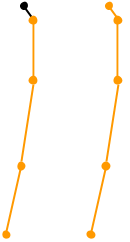
\includegraphics[scale=0.5]{Pictures/ant-segments-repetead-sol1.png}
        \end{column}
        \begin{column}{0.2\textwidth}
        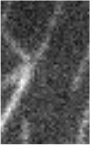
\includegraphics[scale=0.5]{Pictures/NoConsenso2.png}
        \end{column}
        \begin{column}{0.2\textwidth}
        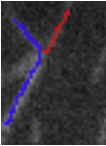
\includegraphics[scale=0.5]{Pictures/NoConsenso3.png}
        \vspace{0.5cm}
        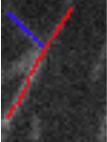
\includegraphics[scale=0.5]{Pictures/NoConsenso4.png}
        \end{column}
    \end{columns}
\end{frame}

\note[itemize]{
    \item La b\'usqueda de soluciones de cada hormiga puede llevar a que dos o m\'as hormigas encuentren soluciones que son muy similares, repitiendo informaci\'on.

}

% \begin{frame}{ACO: Actualizaci\'on de Feromonas (OE 1)}
% \centering
% 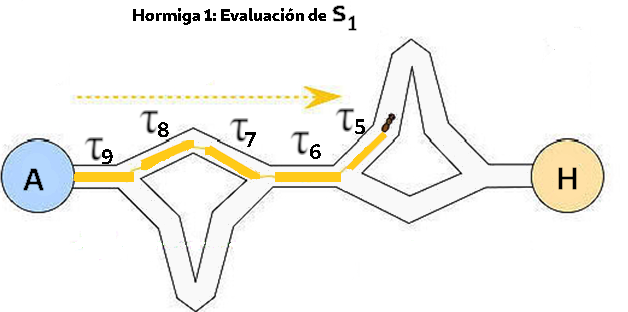
\includegraphics[scale=0.4]{Pictures/ACO-ant-ferom.png}
% \begin{itemize}
%     
% \end{itemize}
% \end{frame}


%\subsection{Anti-feromonas}
\begin{frame}{ACO: Actualizaci\'on de feronomas, uso de Anti-feromonas SAP (OE 1)}
    \centering
    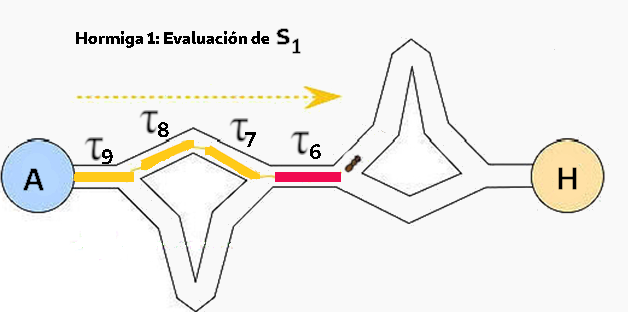
\includegraphics[scale=0.4]{Pictures/ACO-ant-ferom-penalize.png}
    \begin{columns}
        \begin{column}{0.5\textwidth}
            \item Evaluaci\'on de factiblidad de soluciones candidatas $s \in S$
            \item Premiar los caminos de buena calidad
            \item Prop\'osito: Convergencia sobre un camino \'optimo
        \end{column}
        \begin{column}{0.5\textwidth}
            \begin{itemize}
                \item Cambio: $\tau_0 \longrightarrow \gamma$
                \item $\gamma$ es un factor penaliza los caminos de mala calidad
                \item 2 penalizaciones $\longrightarrow \tau_i = 0$ 
            \end{itemize}
        \end{column}
    \end{columns}
    
\end{frame}

\begin{frame}{Problema de Anti-feromonas SAP (OE 1)}
\centering
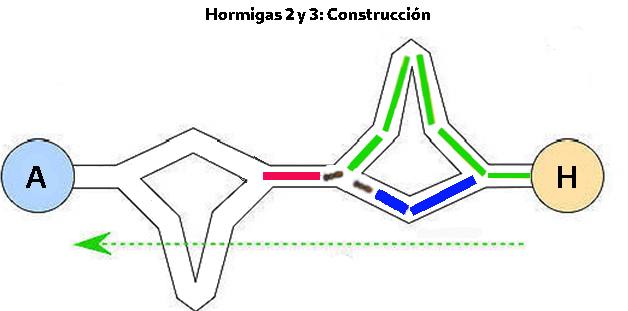
\includegraphics[scale=0.4]{Pictures/ACO-ant-constr-penalize.png}
    \begin{itemize}
        \item Problema: penalizaci\'on puede ocasionar perdida de soluciones factibles
        \item Propuesta: Relacionar penalizaci\'on de $\tau_i$ con $c_i \in s^P$
    \end{itemize}
\end{frame}

\begin{frame}{Anti-feromonas SAP dependientes del camino previo (OE 1)}
    \centering
    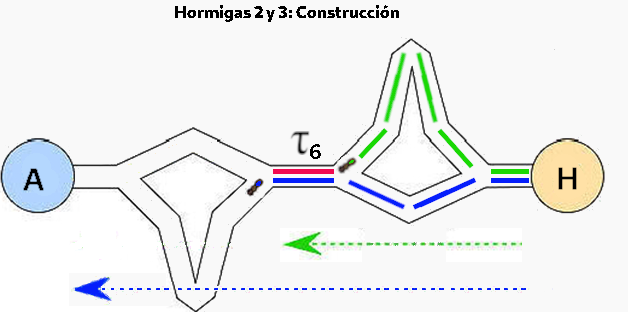
\includegraphics[scale=0.51]{Pictures/ACO-ant-ferom-penalize-seg.png}
\end{frame}


\begin{frame}{Extensi\'on de Anti-feromonas sobre un segmento (OE 1)}
    \centering
    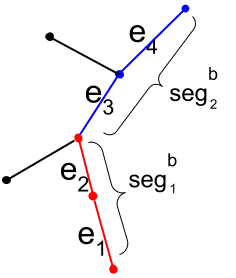
\includegraphics[scale=0.4]{Pictures/ant_segments_simple_case.png}
    \begin{itemize}
        \item Cada arista del segmento forma un \'angulo en el rango $[0, \theta]$ con sus vecinos
        \item Penalizaci\'on de $e_3$ se asocia al $seg^{b}_{1}$, sin perjudicar otros caminos que pasen por $e_3$ pero no por el segmento $seg^{b}_{1}$.
    \end{itemize}
\end{frame}

% \begin{frame}{Anti-feromonas sobre un segmento de una sola arista (OE 1)}
%     \centering
%     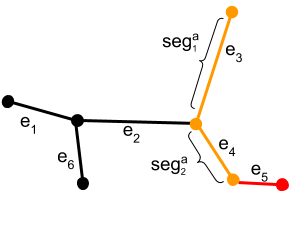
\includegraphics[height=2in]{Pictures/ant_segments_complex_case_B2.png}
%     \hspace{0.1cm}
%     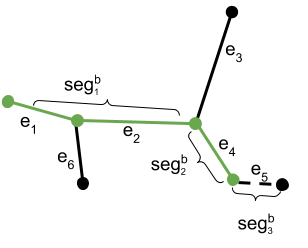
\includegraphics[height=2in]{Pictures/ant_segments_complex_case_B_blocked.png}
% \begin{itemize}
%     \item Segmentos de una sola arista ocasionan mismo problema que se intenta resolver
% \end{itemize}
% \end{frame}

% \begin{frame}{Anti-feromonas sobre un segmento (OE 1)}
% \centering
%     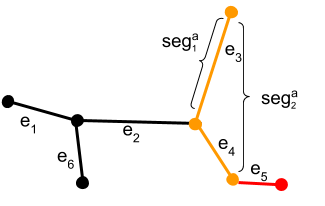
\includegraphics[scale=0.5]{Pictures/ant_segments_complex_case_B2_extended.png}
%     \begin{itemize}
%         \item Se extiende el segmento unitario con el segmento que lo precede
%     \end{itemize}
% \end{frame}

%\subsection{Criterios para la Actualizaci\'on de Anti-feromonas}
\begin{frame}{Anti-feromonas sobre soluciones de calidad intermedia (OE 1)}
\begin{itemize}
    \item Curvatura de una soluci\'on
    \item Magnitud de desplazamiento entre segmentos
    \item Criterio espec\'ifico para neuronas
\end{itemize}
\end{frame}

\begin{frame}{Curvatura de una soluci\'on (OE 1)}
\centering
    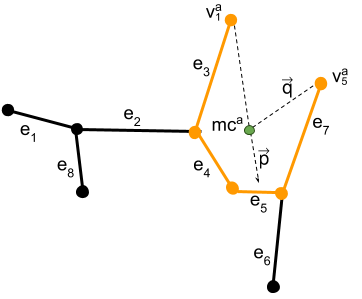
\includegraphics[scale=0.5]{Pictures/ant_curvature_case.png}
    \begin{itemize}
        \item El \'angulo entre la proyecci\'on de $\Vec{p}$ y $\Vec{q}$ debe ser menor a $\theta \times Max\_Axial\_Displacement$ para no descartar la soluci\'on.
    \end{itemize}
\end{frame}

\begin{frame}{Magnitud de desplazamiento entre segmentos (OE 1)}
    \centering
    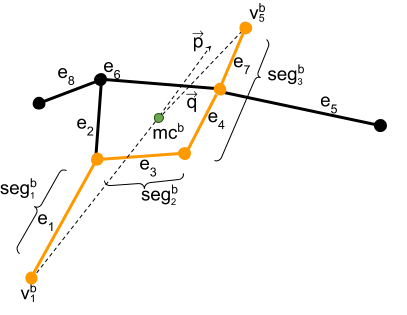
\includegraphics[height=2in]{Pictures/ant_segmentMagnitude_case.png}
    \hspace{0.2cm}
    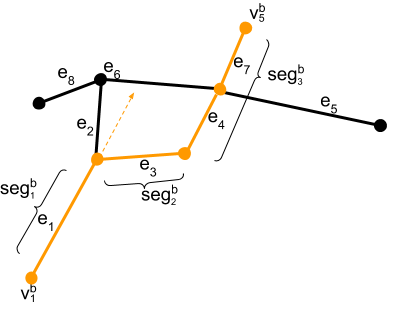
\includegraphics[height=2in]{Pictures/ant_segmentMagnitude_case_2.png}
    \begin{itemize}
        %\item El criterio de curvatura puede no ser suficiente por si mismo
        \item Comportamiento esperado de la rigidez permite descartar soluciones con cambios demasiado pronunciados entre sus segmentos
    \end{itemize}
\end{frame}

%%\subsection{Extracci\'on de informaci\'on para individualizar filamentos}
\begin{frame}{Criterio espec\'ifico para neuronas (OE 1)}
    \begin{itemize}
        \item Se debe validar que los filamentos de una neurona parten del {\bf soma}
        \item  Extracci\'on de informaci\'on: caracter\'isticas geom\'etricas, topol\'ogicas y espaciales
    \end{itemize}
    \begin{columns}
        \begin{column}{0.55\textwidth}
        \centering
        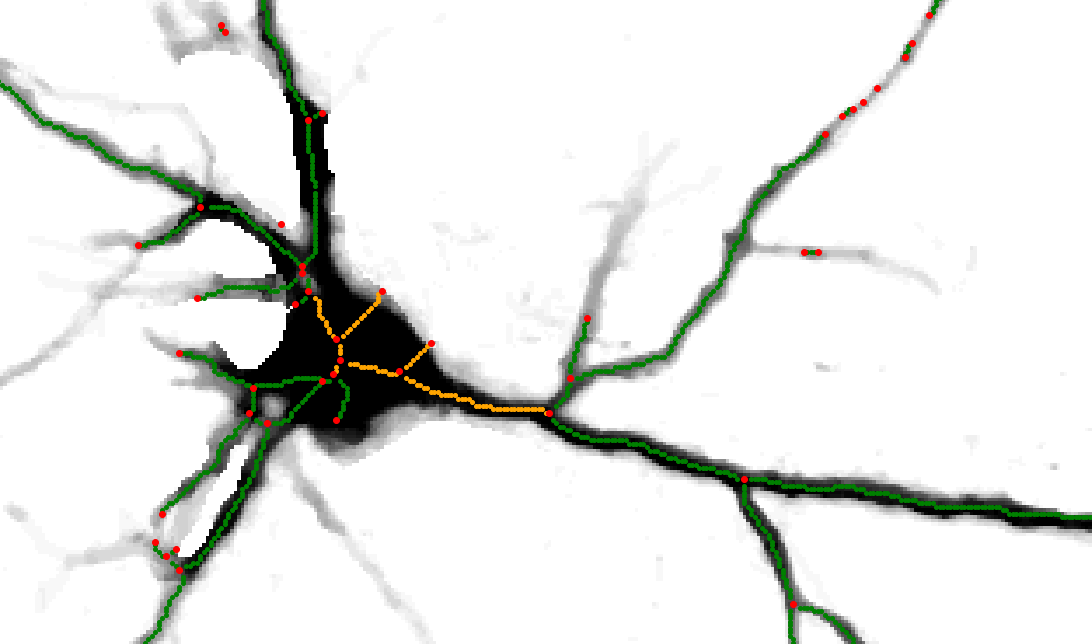
\includegraphics[height=1.7in]{Pictures/Porta183-somaEdges-example2.png}
        \end{column}
        \begin{column}{0.45\textwidth}
            \begin{equation}
                \tau_{ij} \leftarrow
                    \begin{cases}
                     \tau_{ij} \cdot \gamma \text{ si } deg(v^{a}_{n}) = 1,  \\[3ex]
                    
                    \text{0 si } \tau_{ij} \leq 0.25, \\[3ex]
                    \tau_{ij} \quad \text{en otro caso}.
                    \end{cases}
            \end{equation}
        \end{column}
    \end{columns}
    
\end{frame}

% \begin{frame}{Extracci\'on de informaci\'on para individualizar filamentos}
%      \begin{figure*}[h!]
%     \centering
%     \begin{subfigure}[t]{0.48\textwidth}
%         \centering
%         %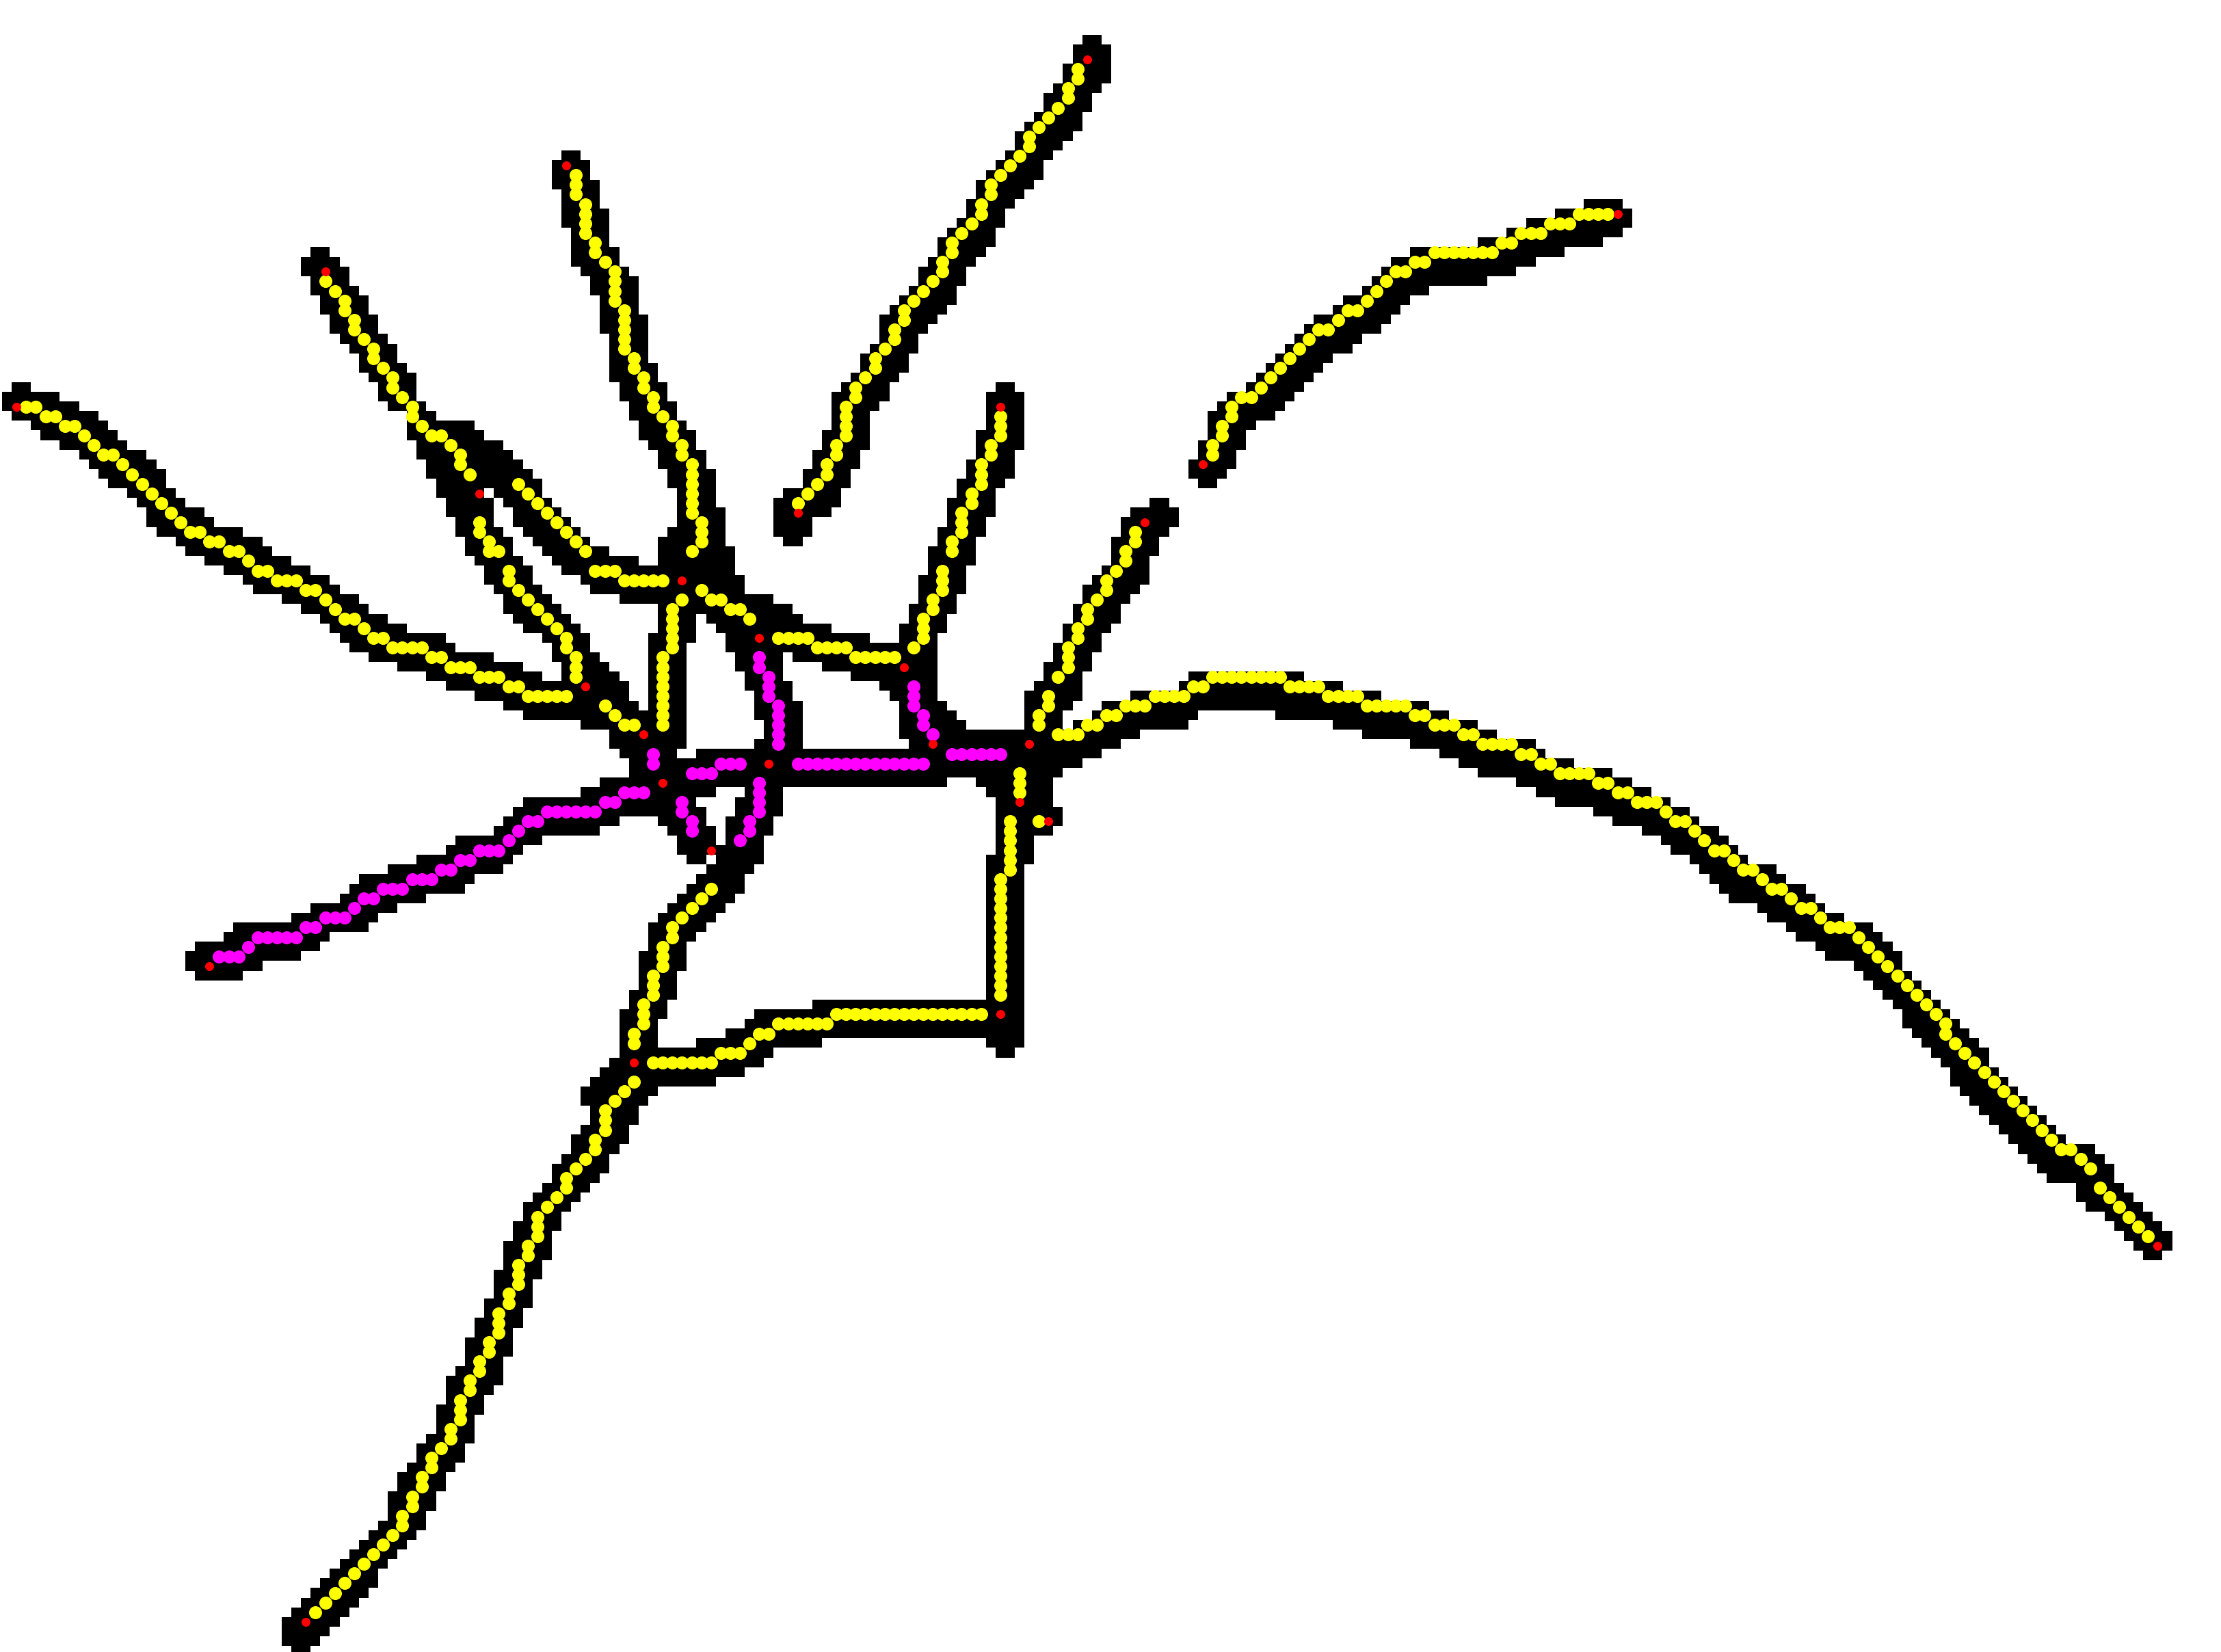
\includegraphics[height=1.5in]{Pictures/50-ROIs-Spinning-Marchantia-somaEdges.png}
%     \end{subfigure}%
%     ~ \hspace{0.1cm}
%     \begin{subfigure}[t]{0.48\textwidth}
%     \centering
%         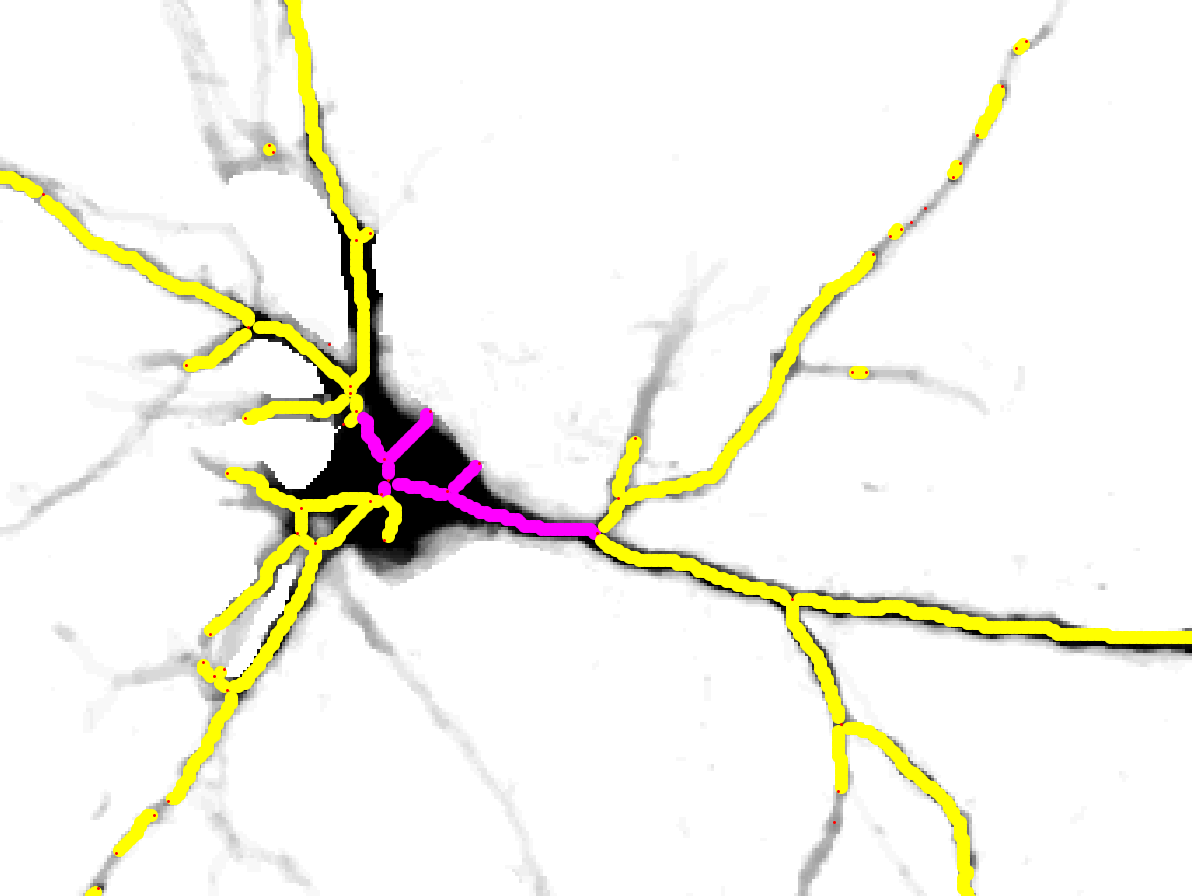
\includegraphics[height=1.5in]{Pictures/Porta18-3a1-somaEdges.png}
%     \end{subfigure}
%     \end{figure*}
%     \begin{itemize}
%         \item Caracter\'isticas geom\'etricas, topol\'ogicas y espaciales
%     \end{itemize}
% \end{frame}